% "THE BEER-WARE LICENSE" (Revision 42):
%
% <timklge@wh2.tu-dresden.de> wrote this file. As long as you
% retain this notice you can do whatever you want with this stuff.
% If we meet some day, and you think this stuff is worth it,
% you can buy me a beer in return - Tim Kluge

\documentclass[12pt,landscape]{article}
\usepackage{multicol}
\usepackage[landscape]{geometry}
\usepackage[utf8]{inputenc}
\usepackage[compact]{titlesec}
\usepackage{listings}
\usepackage{amsmath}
\usepackage{graphicx}

\pagestyle{empty}
\geometry{top=1cm,left=1cm,right=1cm,bottom=1cm}
\setcounter{secnumdepth}{0}

\begin{document}
\footnotesize
\begin{multicols}{3}
\begin{center}
     \Large{\textbf{Einführung in die Medieninformatik}} \\
     \small{Für EMI im 1. Semester beim Bart}
\end{center}


\section{Allgemeines}
\subsection{Aufgabenstellungen}
Berechenbarkeit (Lösen mathematischer Probleme), Unberechenbarkeit, Curchsche These (Gleichwertigkeit aller Maschinenkonzepte), Chomsky-Hierarchie (Zusammenhang Automaten <-> Sprachgrammatik), Programmkomplexität, Programmverifikation
\subsection{Medienkompetenz}
Medialitätsbewusstsein + Medienwissen, Medienspezifisches Rezeptionsmuster, Medienbezogene Genussfähigkeit (Bedürfnis nach Identifikation und Unterhaltung), Medienbezogene Kritikfähigkeit.\\
Medien: Mittel zur Speicherung von Information (Physisch oder Format, Text, Video, Audio, )


\section{Audio}
\subsection{Diskretierung}
\begin{itemize}
\item analoge Audiosignale verlaufen periodisch mit Frequenz ($=$ Tonhöhe, i.d.R. zwischen 20 und 20 kHz), Amplitude ($=$ Lautstärke)
\item Digitalisierung erfolgt über Diskretisierung und Quantisierung:
\begin{enumerate} \item \textbf{Diskretisierung} ist Einteilung der kontinuierliche Zeitachse in diskrete Punkte an denen abgetastet wird (an denen also die Amplitude des Signals gespeichert wird) (wird Angegeben als \textbf{Abtastrate} in Samples pro Sekunde)
\item dabei sollte gelten $f_{\text{abtast}}>2\cdot f_{\text{max}}$ ("Abtasttheorem"), sonst Informationsverluste und Aliasing
\item menschliche Hörschwelle liegt bei 20 kHz; \textbf{Achtung:} liegt z.B. Signal mit $f_{\text{max}}=30$ kHz vor, so sollte dennoch Abtasttheorem eingehalten werden (oder Tiefpassfilter anwenden), da sonst Phantomtöne mit f$<$30 kHz entstehen ($\Rightarrow$ für uns hörbar)
\item \textbf{Quantisierung} ist Speicherung der Amplitudenwerte: dafür steht nur eine begrenzte Bitzahl zur Verfügung, wie präzise man also Amplitudenwerte speichern kann hängt ab von Anzahl verfügbarer bits pro Sample (\textbf{Auflösung}) und min/max Frequenz
\item werden min/max Frequenzen für Digitalisierung falsch gewählt, so kommt es zu Clipping
\item da begrenzt viele bit zur Verfügugn stehen müssen Amplitudenwerte gerundet werden $\Rightarrow$ Quantisierungsrauschen
\end{enumerate}
\end{itemize}
\subsection{PCM}
\begin{itemize}
\item PCM $=$ Pulse Code Modulation, ein verlustfreies Digitalisierungsverfahren, am einfachsten ist \textbf{lineare PCM}
\begin{enumerate}
\item \textbf{analoge Filterstufe}: Tiefpass mit bestimmter Grenzfrequenz (es werden also alle höheren Töne rausgefiltert) $\Rightarrow f_{\text{abtast}}$ muss für Einhaltung des Abtasttheorems nicht ganz so hoch gewählt werden
\item \textbf{zeitliche Abtastung} (=Diskretisierung, siehe Oben)
\item \textbf{Quantisierung} (siehe Oben)
\item \textbf{Codierung} (es wird alles binär gespeichert)
\end{enumerate}
\item weitere Variante: \textbf{D}ifferential \textbf{PCM} d.h. statt den Amplituden an sich wird hier nur Differenz benachbarter Amplituden gespeichert ($\Rightarrow$ max. Kompressionsfaktor 1:2)
\item weitere Variante: \textbf{A}daptive \textbf{DPCM} d.h. DPCM mit Anpassung der Quantisierungsauflösung (je lauter das Signal wird, desto gröber wird quantisiert; siehe auch Quantisierung)
\end{itemize}
\subsection{RIFF WAVE ("WAV")}
\begin{itemize}
\item Containerformat für PCM Daten, diese liegen in Hex vor
\item besteht i.d.R. aus folgenden Chunks: RIFF (12 byte), fmt(8 byte+16 byte), data (8 byte + größe der Rohdaten) 
\end{itemize}
\subsection{Kompression}
\begin{itemize}
\item Informationen können \textbf{redundant} sein (keine neuen Informationen), Informationen können \textbf{irrelevant} sein (nicht wahrnehmbar) $\Rightarrow$ wichtig ist was nicht irrelevant und nicht redundant ist
\item redundant sind z.B. periodische Wiederholungen; irrelevant sind z.B. Frequenzen $>20$ kHz und leise Töne, die durch laute Töne maskiert werden (\textbf{"Mithörschwelle"}); laute Signale maskieren sogar kurzeitig leise Töne die vor/nach dem lauten Signal zu hören wären
\item \textbf{Entropiecodierung} eliminiert Redundanz (verlustfrei), \textbf{Irrelevanz-Codierung/Reduktion} elimiert Irrelevantes (verlustbehaftet) (z.B. durch löschen von Teilsignalen, Anpassung der Quantisierung), \textbf{Dekorrelation} ist Umformung ohne Datenmenge zu ändern
\item \textbf{MP3} = MPEG Layer 3, beansprucht 20-230 kBit/s ($\Rightarrow$ deutlich kleiner als PCM Rohdaten); Signal wird in Fequenzbänder zerlegt, auf diese werden jeweils angewendet u.A. Entropiecodierung, Irrelevanz-Codierung, nichtlineare Quantisierung, Huffman-Codierung
\end{itemize}
\subsection{MIDI}
\begin{itemize}
\item mit dem \textbf{MIDI} Format werden statt Tönen nur Daten zu Instrument, Tonhöhe, Dauer des Anschlags etc. übertragen, woraus ein (evtl. anders klingender!) Ton rekonstruiert wird
\item Verwendung z.B. in Musiksoftware und Synthesizern, das Format wird auch für andere Sachen als Audio verwendet
\item Problem: evtl. Verzögerungen da serielle Übertragung; heute ist Datenübertragung per USB möglich 
\end{itemize}
\subsection{Audioverarbeitung}
\begin{itemize}
\item veränderung der \textbf{Hüllkurve} = Veränderung des Lautstärkeverlaufs, so auch Ein-/Ausblenden (fading)
\item \textbf{Hochpassfilter} multipliziert hohe Frequenzen mit Faktor 1, tiefe mit Faktor 0, dazwischen Faktor zwischen 0 und 1 ($\Rightarrow$ tiefe Frquenzen werden rausgefiltert); umgekehrt für \textbf{Tiefpassfilter}
\item \textbf{Bandpassfilter} analog zu Hoch/Tiefpass aber lässt nur bestimmten Frequenzbereich in der Mitte des Frequenzspektrums durch und filtert höhere und tiefere Frequenzen raus, \textbf{Bandsperre} umgekehrt: filtert mittlere Frequenzen raus
\item \textbf{Dynamikkompression}: laute Stellen werden abgesenkt, leise angehoben
\item Pegeländerungen können zu Über/ Untersteuerung führen (höchste Amplituden liegen weit über/ unter Bereich der quantisiert wird (siehe Quantisierung)); führt zu Clipping (Störsignalen) bei Übersteuerung; führt zu Rauschen bei Untersteuerung
\item \textbf{Resampling}: Signal wird mit anderer Samplefrequenz abgespielt, schneller abgespieltes Signal klingt dann z.B. höher (wie Chipmunks), dieser Effekt kann vermieden werden durch \textbf{Time Stretching} (kurzen Ausschnitt wiederholt abspielen)
\end{itemize}
\subsection{Klangsynthese}
\begin{itemize}
\item Anschlagsverhalten wird per Hüllkurve in 4 Schritten nachgebildet: Attack (wie schnell wird der Ton direkt nach dem Anschlag lauter), Decay (wie schnell erreicht er gleichbleibende Lautstärke), Sustain (Lautstärke beim Aushalten), Release (Loslassen)
\item \textbf{Wave-Table Verfahren}: es wird zum Beispiel Datei für den Laut "E" oder einen Klavierton gespeichert und bei Bedarf abgespielt, gleiches dann für alle anderen Laute/Töne 
\item \textbf{Additive Synthese}: jede Funktion kann als unendliche Summe von cos/sin dargestellt werden $\Rightarrow$ durch endliches addieren von solchen Funktion kann gewünschtes Signal angenähert werden 
\item \textbf{subtraktive Synthese} nimmt durch Oszillator erzeugtes Signal und verändert dieses durch Filter
\item \textbf{FM-Synthese} (z.B. bei alten Keyboards) modulieren von Trägerfrequenz durch Modulationsfrequenz, resultierender Klang entspricht keinen akustischen Instrumenten
\item Synthesizer erstellen durch GUI oder Skript möglich 
\end{itemize}


\section{Video}
\subsection{Historie}
\begin{itemize}
%\item Laterna magica (1671): Ähnlich zu Diaprojektor, mit Glasscheiben, die gegeneinander bewegt werden
%\item Daumenkino (1868), Lebensrad (1833)
%\item Wundertrommel: Streifen mit Zeichnungen in einem drehenden Kreis, Bild wird durch Schlitze beobachtet - Praxinoskop: Spiegel im Inneren, die auf die Innenseite des drehenden Kreises zeigen und so das gerade vorbeilaufende Bild zeigen, Rotoskop: Daumenkino mit Fotos
\item Zelluloidfilm ab 1888 (Photoemulsion auf Zelluloid): Verschiedene Filmformate, heute \textbf{35mm, 24 Bilder / Sekunde}, 1km film ergibt ca. 36,5 min
\item Kinemacolor (1906): 32 Bilder / sek, 16 rot, 16 grün mit rotierendem Filter
\item Technicolor (1917): Aufspaltung mit Prisma auf 3 Filme
\item Agfacolor (1932): als Farbfilter wirkende Körner auf dem Papier
\item Edison Phonograph (1877): Nadel schreibt Ton auf Walze mit
\item Lichttonverfahren (1922): Lichtdurchlässigkeit proportional zur Amplitude des Tonsignals
\item Später: Kombination mit Magnetton (vgl. Tonband, Cassette)
\item 4-Kanalton wird als Matrix in die Lichtkanäle moduliert, Dolby 5.1 Surround auf CD oder digital in Filmperforation, 8-Kanal-SDDS komprimiert digital auf Filmaußenrand
\item Interaktive Filme: Mehrere Perspektiven werden aufgenommen und durch den Benutzer gewechselt
\item Rendering: Berechnung jedes Bildes durch Rechner (Animationsfilm)
\item Kamera (Edison: Kinematograph 1891). Unbelichteter Film wird von Spule in Kamera gerollt, ein Bild belichtet, Blende verdeckt das Bild, Film wird auf zweite Spule gerollt und anschließend entwickelt
\item Projektoren für 35mm: Kinetoscope (1892 Edison) mit einem Betrachter, ab 1895 auf Leinwand
\item Projektor in modernem Kino: Film auf 3 Tellern gewickelt, rein ins Projektor, raus auf freien Teller
\item Digitalprojektor: digitales Bild wird gelesen, Lampe wird extra gekühlt
\subsection{Formate}
\item Flüssige Bewegung ab ca. 20 FPS, Film: \textit{\textbf{24 Hz}}
\item Flimmern: Bei Dunkelpausen zwischen Bildern, dadurch unangenehmes Flackern
\item Flimmerverschmelzungsfrequenz ca. 50 Hz, steigt mit Helligkeit
\item Bilder zweifach projiziert, Verdopplung der Dunkelpausen, Flimmerfrequenz 48 Hz
\item Computermonitore: hohe Helligkeit, geringer Abstand, hohe Aufmerksamkeit. Frequenz muss mindestens 72 Hz sein
\item Keine Dunkelpausen bei TFT-Displays, dadurch kein Flimmern
\item Helligkeitsempfindung unterstützen, abhängig vom Zustand des Auges (Auge kann sich an Leuchtdichteunterschiede anpassen, von mondloser Nacht zum sonnenbeschienenden Schneefeld in 30 min). Das angepasste Auge kann ca. 200 Helligkeitswerte unterscheiden
\item Fernsehen: Streulicht schränkt Kontrastwahrnehmung ein, Umfeldleuchtdichte sollte ca. 10 \% der Spitzenleuchtdichte des Bildschirms betragen
%ab hier wieder wichtig
\item \textbf{Aliasing}: Treppenstufen und Geisterfrequenzen bei Abweichung von abgetastetem und abtastenden Raster
\item \textbf{Zeitliches Aliasing} (Wagenradeffekt): Wagenrad scheint sich rückwärts zu drehen bei zu geringer Abtastfrequenz, Stillstand falls genau um 90 Grad  verdreht. Vermutlich durch neuronale Adaption verursacht
\item \textbf{Videosignal (s/w analog): Zeilenweise Abtastung der Helligkeitswerte, serielle Übertragung der Bildpunkte, synchrone Darstellung auf dem Monitor}
\item \textbf{Progressiv}: Ganzes Bild für Zeile für Zeile übertragen
\item \textbf{Interlaced}: 2 Halbbilder werden nacheinander übertragen und ergeben zusammen ein Vollbild. Das erste Bild beschreibt nur jede zweite Zeile etc. Ursprünglich zur Reduktion von Bildflimmern entwickelt (50 Hz bei Röhrenmonitoren)
\item 100Hz-Röhrenfernseher und LCDs sowie Plasmafernseher zeichnen progressiv, dadurch \textbf{Umrechnung} des TV-Signals erforderlich
\item \textbf{Weave}: \textbf{Gleichzeitige Darstellung der Halbbilder.} Funktioniert bei TV nicht, da die Halbbilder zeitlich versetzt aufgenommen werden, führt zu Kammeffekt
\item \textbf{Unschärfe}: \textbf{Weave mit Weichzeichnen}
\item \textbf{Motion Compensation:} \textbf{Weave}, wobei ungerade Zeilen an gerade Zeilen \textbf{angepasst} werden \textbf{(aktuell)}
\item \textbf{Bobbing: }Jedes Halbbild wird durch \textbf{interpolation} zu einem Vollbild erweitert, um 50 Hz zu erreichen. Dadurch \textit{wackelt das Bild}, da erste und letzte Zeile jeweils ohne Nachbar sind
\item \textbf{Blending:} \textbf{Bobbing}, wobei \textbf{beide Halbbilder} zum Vollbild ergänzt werden und dann der \textbf{Mittelwert} zwischen beiden Bildern genommen wird
\item Analoge Formate
\begin{itemize}
    \item Analoges Fernsehen ohne Zwischenspeicherung arbeitet mit Zeilen (progressive) und Halbzeile (interlaced) 
    \item \textbf{BAS}: Helligkeit auf 75 \% Signalamplitude skaliert, Austastung durch Zeilenrücklauf (100 \% Amplitude für 5 Mikrosekunden), Bildsynchronisation durch volle Amplitude für 10 Mikrosekunden
    \item \textbf{FBAS}: Farbsignale werden überlagert
    \item \textbf{Komponentenvideo}: Getrennte Übermittlung von drei Farbkanälen (RGB, YUV oder YIQ)
    \item \textbf{Y/C-seperiertes} Video: Trennung von Helligkeit und Chrominanzsignalen
    \item Europäisches Standardsignal \textbf{PAL }(Phase Alternate Line System): \textbf{interlaced FBAS} in YUV, Auflösung 833x625 Pixel, 720x576 sichtbar, 50 fields = \textbf{\textit{25 fps}}; Bandbreite Y: 5,5Mhz, U/V: 1,8 Mhz
    \item \textbf{NTSC }(National Television Systems Committee): US Standard, \textbf{Interlaced FBAS} in YIQ, 700x525 Pixels, \textit{\textbf{29,97 fps},} ohne Kontrolldaten 485 Zeilen, wovon 480 nutzbar sind
    \item \textbf{Secam }(Sequential Couleur avec Memoire): wie PAL mit Bandbreiten 6/2/2 (Y/U/V)
    \item NTSC in Amerika, PAL in Europa, Australien, Asien, Secam in Frankreich / Russland
\end{itemize}
\item Digitale Formate
\begin{itemize}
    \item Digitale Videos unterstützen weitere Seitenverhältnisse und korrigieren nichtquadratische Pixel
    \item Digitales Fernsehen wird über Funktechniken (Antenne, Satellit) und Kabel verbreitet
    \item DVB: Digital Video Broadcast, MPEG2-basiert, Senden als Stream, MPEG Digital Storage Command Control (DSM-CC) für Interaktivität. DVB-C (Cable), DVB-T (Trerristisch über Antenne), DVB-S (per Satelit), Container nach \textbf{Objektkarussel} transportiert \textbf{Audio, Video und Daten}. DVB-H für Verteilung über Mobilfunk nicht mehr verbreitet
\end{itemize}
%\item HbbTV (Hybrid Broadcast Broadband TV): DVB mit CE-HTML, JavaScript und Medieninformation (JavaScript zur Zeit nicht standardisiert), OIPF Medienformate verschieden. TV-Programm wird mit Signal mitgeliefert, Application Information Table (AIT) wird bei jedem Sendersignal mitgeliefert und enthält URL für Aufruf beim Drücken der roten Taste
\item \textbf{Bildebenen}: schwarzer Hintergrund, Video, Untertitel / Gebärden, HbbTv, Geräteoberfläche (Uhrzeit, Lautstärke). Anwendungen werden über HTTP vom Sender ermittelt.
\item \textbf{Seitenverhältnis}:TV 4:3 (1.33:1), HDTV 16:9 (1.78:1), 21:9 (2,33:1); Je nach analogem Format werden die einzelnen (digitalen) Pixel entsprechend nichtquadratisch gespeichert \textit{Digitale Videos unterstützen weitere Seitenverhältnisse und korrigieren nichtquadratische Pixel}
\item \textbf{Digitales Video}: Bilder werden als Sequenz gesendet. Ein Videostream besteht aus Bildern und Teilbildern, sowie Ton.
Bilder bestehen aus Pixeln. Pixel haben eine Farbe.
\subsection{Komprimierung}
%\item Farbwahrnehmungsbezogenes Chroma-Subsampling $Y:C_R:C_B$, Y-Abtastung 3 Mhz, $C_R$ und $C_B$-Abtastraten ev. geringer, Räumliche Position wird angedeutet
%\item AVI: Containerformat für beliebigen Codec
%\item DV-Standard bei Camcordern (DCT, D1, D2..., Digital Betacam), CCIR 601 o. ä.
%\item MJPEG: JPEG-basierte Kompression der Vollbilder, nicht standardisiert
%\item MPEG: Standard
\item Diskretisierung (Abtastung)
\begin{itemize}
    \item \textit{Diskretisierung muß Farbe in historischem Schwarzweiss-Verfahren integrieren}
    \item \textbf{4:1:1} Farbsignal nur bei jedem 4.Pixel, dafür aber in beiden Halbbildern horizontal verschoben abgetastet.
    \item \textbf{4:2:0} Farbsignal nur bei jedem zweiten Halbbild und nur in halber Auflösung abgetastet
    \item \textbf{4:2:2} Jedes Pixel wird nach Luminanz (Y) und jedes 2. nach den Rot- und Blaudifferenzen (Cr und Cb) abgetastet.(für professionelles digitales Video)
    \item \textbf{4:4:4} Jedes Pixel, sowohl in Luminanz wie in den Blau- und Rotdifferenzen wird abgetastet; (Hochqualitatives digitales Format)
\end{itemize}
\item \textbf{CODEC}: bezeichnet ein Algorithmenpaar: \textbf{Compressor} komprimiert die Videodaten; \textbf{Decompressor} stellt Ursprung wieder her; meist sind dabei Informationen verloren gegangen
\item Komprimierungstechnik: 
\begin{itemize}
    \item \textbf{Redundanz Reduktion}: Verzicht auf mehrfach vorhandene Information(z.B. räumlich, zeitlich ); (verlustfrei)
    \item \textbf{Irrelevanz Reduktion}: Verzicht auf kaum erkennbare Signalanteile (verlustbehaftet)
\end{itemize}
\item Bei Video besonders sinnvoll, Differenz zwischen zwei Bildern zu berechnen (vgl. \textbf{DPCM})
\item \textbf{H.261}: Video-Telefonie über ISDN (Bandbreite 64 kbit/s mal Kanal), weniger als 150ms Verzögerung durch Kompression / Dekompression, CIF / QCIY, YCrCb 4 : 2 : 0, Kompression auf 1,5Mbit / s (24x ISDN)
\item \textbf{H.263}: Weglassen unwichtiger Teile und Verringerung der Bittiefe, halbe Datenrate
\item \textbf{Intraframes} (JPEG codiert): 16x16 große Blöcke, Unterteilung in 8x8-Blöcke für Helligkeit und zwei Blöcke für Chromakanäle, DCT mit anschließender Huffmann-Codierung
\item \textbf{Predicted Frames}: Unterteilung in 16x16 Blöcke, für jeden Block Suche nach "Best Match" im vorherigen Frame, \textbf{Differenzcodierung}
\item \textbf{MPEG} (Moving Pictures Experts Group): Standard für komprimiertes Speichern von Audio und Video. MPEG-1 (1992, nur progressiv für Videos), MPEG-2 (1993, TV, HDTV), MPEG-3 (HDTV, in MPEG-2 integriert), MPEG-4 (laufende Entwicklung), MPEG-7 (DescriptionInterface), MPEG-21 (Digital Multimedia Framework)
\item \textbf{Sequence:} Alle Bilder vom $s_{header}$ bis zum $s_{end}$
\item \textbf{GOP:} Group of Pictures zwischen 2 GOP-Headern
\item \textbf{Picture}: Field (Halbbild, d.h. jede zweite Zeile) od. Frame (Vollbild)
\item \textbf{Macroblock}: 16 x 16 Pixels
\item \textbf{Slice}: 16 Zeilen
\item \textbf{Block}: 8 x 8 Elemente (Luminanz / Chrominanz / DCT-Koeff.)
\item \textbf{Sample}: Einzelner Helligkeitswert eines Pixels
\subsection{MPEG}
\item Bei MPEG-1 werden \textbf{B-Frames} eingeführt, die von vorne und hinten interpoliert werden (\textbf{Macroblockweise} aus nächstem und vorherigen vorhergesagt; \textbf{Differenz} mit DCT und Huffmann-Kodierung), I-Frames JPEG-kodiert, ansonten wie H.261
\item MPEG Datenstrom
\begin{itemize}
    \item \textbf{Audio}: Gliederung in Frames (Folge von Abtastwerten), Audio Access Units (kleinste für sich voll dekodierbare Einheit) und Slots (1 - 4 Byte).
    \item \textbf{Video} aus 6 Schichten: Sequence Layer, Group of Pictures layer (Abfolge der verschiedenen Bildtypen), Picture layer (kodierte Einzelbilder), Slice Layer (Ebenen, Komponenten) eines Bildes, Macroblock Layer (Makroblöcke), Block Layer (Einzelblöcke)
\end{itemize}
\item MPEG-2 zu MPEG-1: Best-Match-Suche auch nach Fields, Makroblöcke Farb-Subsampling von 4 : 2 : 2, 4 : 4 : 4, die Frame-Größe kann bis zu $16383^2$ Pixel betragen, nichtlineare Quantisierungstabelle
\item Verschiedene Profile (High Level: FullHD, Main Level: HD), in höheren Profilen \textbf{räumliche Skalierbarkeit} (Datenstrom kann in verschiedenen Auflösungen gezeigt werden), \textbf{Zeitliche Skalierbarkeit} (Datenstrom adaptiv zu Veränderungen der Bandbreite)
\item \textbf{MPEG-1} bis HD (CD-ROM, Digital Storage Media); (1,5 Mbps); 352x240, 720x480; Stereo CD 
\item \textbf{MPEG-2} DVD, Broadcast, HDTV, (4,6 Mbps); 176x144, 352x288, 1280x720; Surround Sound
\item \textbf{MPEG-4} für TV, Virtual Games, Streaming [...]; (20 Kbps - 6 Mbps); 176x144, 352x288, 720x480, 1280x720; Sprache, Musik, CD
\item MPEG-4: Kodierung von Szenen von audiovisuellen Objekten, Kombination natürlicher und synthetischer Medien-Objekte, Prinzip unabhängig von Bitrate (low bitrate bis lossless)
\end{itemize}
\subsection{YUV}
\begin{itemize}
\item Farbwahrnehmungsbezogenes Chroma-Subsampling $Y:C_R:C_B$, Y-Abtastung 3 Mhz, $C_R$ und $C_B$-Abtastraten ev. geringer, Räumliche Position wird angedeutet
\item AVI: Containerformat für beliebigen Codec
\item DV-Standard bei Camcordern (DCT, D1, D2..., Digital Betacam), CCIR 601 o. ä.
\item MJPEG: JPEG-basierte Kompression der Vollbilder, nicht standardisiert
\item MPEG: Standard
\item Bei Video besonders sinnvoll, Differenz zwischen zwei Bildern zu berechnen (vgl. DPCM)
\item H.261: Video-Telefonie über ISDN (Bandbreite 64 kbit/s mal Kanal), weniger als 150ms Verzögerung durch Kompression / Dekompression, CIF / QCIY, YCrCb 4 : 2 : 0, Kompression auf 1,5Mbit / s (24x ISDN)
\item H.263: Weglassen unwichtiger Teile und Verringerung der Bittiefe, halbe Datenrate
\item Intraframes (JPEG codiert): 16x16 große Blöcke, Unterteilung in 8x8-Blöcke für Helligkeit und zwei Blöcke für Chromakanäle, DCT mit anschließender Huffmann-Codierung
\item Predicted Frames: Unterteilung in 16x16 Blöcke, für jeden Block Suche nach "Best Match" im vorherigen Frame, Differenzcodierung
\item MPEG (Moving Pictures Experts Group): Standard für komprimiertes Speichern von Audio und Video. MPEG-1 (1992, nur progressiv für Videos), MPEG-2 (1993, TV, HDTV), MPEG-3 (HDTV, in MPEG-2 integriert), MPEG-4 (laufende Entwicklung), MPEG-7 (DescriptionInterface), MPEG-21 (Digital Multimedia Framework)
\item Sequence: Alle Bilder vom $s_{header}$ bis zum $s_{end}$
\item GOP: Group of Pictures zwischen 2 GOP-Headern
\item Macroblock: 16 x 16 Pixels
\item Slice: 16 Zeilen
\item Block: 8 x 8 Elemente (Luminanz / Chrominanz / DCT-Koeff.)
\item Sample: Einzelner Helligkeitswert eines Pixels
\item Bei MPEG-1 werden B-Frames eingeführt, die von vorne und hinten interpoliert werden (Macroblockweise mit DCT und Huffmann-Kodierung), I-Frames JPEG-kodiert, ansonten wie H.261
\item Audio: Gliederung in Frames (Folge von Abtastwerten), Audio Access Units (kleinste für sich voll dekodierbare Einheit) und Slots (1 - 4 Byte).
\item Video aus 6 Schichten: Sequence Layer, Group of Pictures layer (Abfolge der verschiedenen Bildtypen), Picture layer (kodierte Einzelbilder), Slice Layer (Ebenen, Komponenten) eines Bildes, Macroblock Layer (Makroblöcke), Block Layer (Einzelblöcke)
\item MPEG-2 zu MPEG-1: Best-Match-Suche auch nach Fields, Makroblöcke Farb-Subsampling von 4 : 2 : 2, 4 : 4 : 4, die Frame-Größe kann bis zu $16383^2$ Pixel betragen, nichtlineare Quantisierungstabelle
\item Verschiedene Profile (High Level: FullHD, Main Level: HD), in höheren Profilen räumliche Skalierbarkeit (Datenstrom kann in verschiedenen Auflösungen gezeigt werden), Zeitliche Skalierbarkeit (Datenstrom adaptiv zu Veränderungen)
\item MPEG-1 bis HD (1,5 Mbps), MPEG-2 für DVD oder Broadcast oder HDTV: 4,6 Mbps, MPEG-4 20 Kbps - 6 Mbps für TV, Virtual Games, Streaming [...]
\item Neue Interaktivität in MPEG-4 gewünscht
\item MPEG-4: Kodierung von Szenen von audiovisuellen Objekten, Kombination natürlicher und synthetischer Medien-Objekte, Prinzip unabhängig von Bitrate (low bitrate bis lossless)
\item 3D-Szenengraph: Objektbaum
\item X3D, VRML, OpenGL: Rendering-Pipeline (Tesselation, Transformation, Sichtbarkeit, Beleuchtung, Projektion, Clipping, Transformation in affine Koordinaten, Viewport mapping, Scan conversion, Verdeckung, Scissoring, Shading / Texturisierung, AntiAliasing)
\item VRML: "SVG in 3D" ohne XML, z. B:
\begin{lstlisting}
#VRML V2.0 utf8
Shape {
geometry Box{ size 2 2 2}
}
\end{lstlisting}
\end{itemize}
\section{Multimodale Systeme}
Multimodale Systeme nutzen mehr als einen Sinneskanal zur Wahrnehmung beim Menschen. Dadurch Verbesserung der Intuition und Erhöhung der Robustheit eines interaktiven Systems z. B. durch Einbringung von Lippenbewegungen, Kommunikation kann barrierefreier gestaltet werden.
\begin{itemize}
\item Pipeline zur Wahrnehmung: Stimulation, sensorischer Kurzzeitspeicher, Wahrnehmung, Entscheidungsfindung, Reaktion, ggf. Gedächtnisspeicherung. Aufmerksamkeit ab Wahrnehmung nötig.
\item Beispielsweise Datenhandschuh, Joystick
\end{itemize}
\subsection{Stereoskopische Ausgabe}
\begin{itemize}
\item Shutter-Brillen, Head Mounted Display (Problem: Cyber-Sickness weil Bewegungen unnatürlich)
\item Head Mounted Display: Kopfhörer, Positionssensoren liefern Daten über Lage und Blickrichtung
\item Autostereoskopische Techniken: z. B. 3D-LCD-Display mit Linsensystem, führt Kopfbewegungen mit Head-Tracking-System nach (Brechwinkel bedingen Abstand), Objekte können vor und hinter dem Display liegen
\item Autostereoskopische Displays sind noch nicht ausgereift: Meist nur ein oder zwei Betrachter, nur Raumillusion, feste Betrachtungsposition, "Blick durch Fenster" (nicht sehr realitätsnah), Objekte, die nur von einem Auge gesehen werden, müssen ausgeblendet werden, noch zu reaktionslahm
\item Polarisierte Lichtquellen für 3D: Bild wird polarisiert statt durch Farbfilter überlagert, je ein Auge sieht horizontal oder vertikal polarisiertes Licht
\item STB: Interaktiver Empfänger für Fernsehen und Internet. Bindeglied zwischen HiFi, TV, PC etc und Internetz. Standards für APIs, Netzprotokolle, Medienformate. Unterschiedliche Hardwarekonzepte, aber meist Tunermodul, Demodulator, Prozessor, MPEG2-Decodierer, Demultiplexer, Backchannel-Controller, Descrambler, Schnittstellen-Controller, Audio DAC, Entschlüsselungssystem (Conditional Access)
\end{itemize}


\section{Processing}
\begin{itemize}
\item Variablendeklaration: TYP NAME=WERT (Variablennamen immer klein schreiben)
\item Felder: TYP[ ][ ] NAME = \{WERT1, WERT2, ...\}, \{WERT\_A, WERT\_B, ...\} (eindimensional oder mehrdimensional möglich); Zuweisung über NAME[1][0]=45; (Elemente von 0 beginnend nummeriert)
\subsection{Ausgaben}
\item print(); Ausgabe auf der Konsole; println() mit anschließendem Zeilenumbruch
\item Kommentare mit \textbf{//} oder mehrzeilig mit \textbf{/*...*/}
\item Formen: line(x1, y1, x2, y2); triangle(x1, y1, x2, y2, x3, y3); rect(x, y, breite, hoehe); ellipse(xM, yM, durchmesserBreite, durchmesserHoehe);
\item Zeichenmodi: rectMode(CORNER): normal linke obere Ecke als Bezugspunkt; rectMode(CENTER): Mittelpunkt als Bezugspunkt; rectMode(CORNERS) zwei EckPUNKTE angeben; (für ellipseMode ist CENTER standard, CORNER[S]arbeitet mit umgebenden Rechteck
\item Farben: fill(0-255) für Graustufen; fill(R,G,B) in 8bit(0-255) erwartet; gilt für alle folgenende gezeichneten Formen; (weiterer Wert bei fill() Methode für Transparenz) 
\item Hintergrund: size(x,y) legt Breite, Höhe fest; background(R,G,B) Farbe des Hintergrundes festlegen (auch mit Graustufen mgl. s. o.); befehl übermalt gesamten Zeichenbereich
\item Text: text(string, basisX, basisY); [basis=linke untere Ecke]; textSize(0-$\infty$) Textgröße in pt; textAlign() CENTER, LEFT, RIGHT Ausrichtung des Textes 
\item String (Bsp. s): s.length() gibt Länge des Strings zurück; s.equals(s2) prüft Strings auf Inhaltsgleichheit (nicht = verwenden überprüft Speicheradressen); s.substring(0,5) gibt Teilstring (start inklusive, ende exklusive) zurück (start bei 0) im Bsp. die ersten 5 Zeichen von s
\subsection{aktiver Modus}
\item benötigt \textit{void setup()\{\}} und \textit{void draw()\{\}} (Endlosschleife bis Programm abbricht) Methoden
\item framerate() in 1/s für draw Methode im setup Teil festlegbar
\item Mauseingaben: Variablen \textbf{mouseX} und \textbf{mouseY} beinhalten aktuelle Position der Maus \textit{pmouseX, pmouseY} enthalten Position der Maus in vorheriger draw "Runde"
\item Tastatur Eingaben: \textit{void keyPressed()\{\}} methode beinhaltet Variable Key mit gedrückter Taste (Unterscheidung über Switch Anweisung hilfreich) (ebenso \textit{void mousePressed()\{\}}) (!!funktioniert nur im aktiven Modus (setup und draw))
\item Zufall: random(10) gibt zufällige Zahl zw. 0 und 9
\subsection{Audio}
\item \textit{import processing.sound.*;} Importiert Soundbibliothek 
\item SinOsc osc; Deklaration einer Oszillator Variable; osc = new SinOsc(this); Speicher von osc wird intitialistiert; (meist in setup ausgeführt)
\item osc.play(freq, amp); startet Ausgabe eines Tons (osc.stop soppt Ton)
\item osc.amp(amp) verändert Amplitude[0,1]; osc.pan(pan) verändert links rechts[-1,1]; osc.freq(freq) verändert Frequenz[hörbarer Berreich];
\end{itemize}


\section{Java}
\subsection{Java Programmierung}
\begin{itemize}
\item Java ist objekt-orientiert (parallele Progammierung ist leicht möglich)
\item Java ist dynamisch Speicherbedarf wächst und schrumpft automatisch
\item Übersetzen des Quellcode in Bytecode:
\begin{enumerate}
    \item Eingabe von Quellcode (erzeugt Quellcode Datei)
    \item Übersetzen in Bytecode (erzeugt seperate Bytecode Datei [Prozessor lesbare .class Datei]) (bei Fehler gehe zu 1)
    \item bei Erfolg: ausführen des Bytecodes (bei Fehler gehe zu 1) 
\end{enumerate}
\item Bytecode für alle OS gleich; Unterscheidung im jeweiligen Interpreter 
\item Hauptbestandteile: 
\begin{itemize}
    \item Methode: ist eine Folge von Anweisungen; werden aufgerufen (können sich selbst aufrufen(rekursion)); werten Parameter aus; können vererbt werden(nur bei objektorientiert)
    \item \textit{main}-Methode: einzigartig in jedem Programm; legt Beginn des Programms fest; wird vom Interpreter als erstes im Bytecode gesucht 
    \item Klassen: sind Vorlagen für Objekte (mit \textit{new} werden Objekte erzeugt); Objekte haben Attribute(Eigenschaften) und führen Methoden aus
    \item Blöcke: fassen Folgen von Anweisungen zusammen; legen den Namensraum für Variablen fest; Verschachtelung mgl.; in geschweiften Klammern
    \item Anweisungen
    \item Kontrollstrukturen: If, While, For(Foreach), Do, Switch, Kontrolltransfer-Anweisungen(break: beende Anweisungsfolge (beendet eine oder mehrere verschachtelte Schleifen), continue: beendet in einer Schleife sofort einen Durchlauf, return: beendet Anweisungsfolg einer Methode, (throw: später))
    \item Modifiers: \textit{public, static}
    \item Package: enthält(Quellcode und Bytecode) einer oder mehrere Klassen, die sich einen gemeinsamen Geltungsbereich (Namespace) für Klassen teilen; Klassennamen müssen nur in einem Package eindeutig sein; über \textit{import} einzelne Klassen importierbar 
    \item Kommentare: //..., /*...*/
    \item reservierte Worte: \textit{claas}, alle Modifiers,... dürfen nicht für Variablennamen o.Ä. verwendet werden
\end{itemize}
\subsection{Android Apps}
\item Android ist linuxbasiert; Apps laufen auf optimierter Java VM für mobile Prozessoren; Apps kommunizieren miteinander (durch Intents)) 
\item Apps bestehen aus Modulen für interaktion des Nutzers mit Daten(Activities); beenden sich selbst über ständig prüfende "Abbruchschleife"
\item \textbf{Entwicklungsprozess}: Setup (IDE wählen, SDK, virtuelle Geräte einrichten); Entwicklung (Quellcodes, Ressourcen, Manifest); Debugging(ADB, logs, Geräte per USB testen); Veröffentlichung(Release, Signatur, App Store)
\item Quellcode $\Rightarrow$ Bytecode: Android Package Datei (ausführbare Datei) enthält: Datei, (formatierte)Ressourcen, AndroidManifest.\textbf{xml} (beschreibt: SDK Version, packages, Activities, Icon, Stil)
\item Daten $\Rightarrow$ Medien: (von unten) [Bits und Byte] [Sensordaten, Prozessor] [Netzwerk, Protokolle] [Ressourcen, Medien, Codec] [GUI] [App] nur oberen 3 Komponenten in der App sichtbar
\subsection{Smartphone}
\item Ausgabetechnik: Display, Lautsprecher, Vibrationsmotor
\item Eingabetechnik: Touchscreen, Uhr(am Kernel), Akkumulator, Sensoren(Mikrofon, Kamera, Gyroskop, Beschleunigungssensor, Kompass, Thermometer, Näherungssensor, Lichtsensor, GPS, Barometer,...)
\item Kabel-/Funkschnittstellen: USB, Wifi, Bluetooth, NFC(RFID)
\item MEMS-Sensor: Bewegung einer Reonanzmasse verändert Kapazität messbar (Beschleunigungen, Kreisbewegungen); Anwendung: Schrittzähler, Anzeigeausrichtung ändern, Bewgung in Räumen
\item Näherungssensor: Reflektion von Infrarotlicht auf kurzen Distanzen(z.B beim am Ohr halten); Anwendung: Display ausschalten bei Telefonat, Gestensteuerung
\item Magnetsensor: Messung des Erdmagnetfeldes im 3 dimesionalen Raum (Hall-Effekt); Anwendung: VR Brillen, präzisere Lagebestimmung
\subsection{Technologien zur Barrierefreiheit von Apps}
\item 4 Prüfkriterien:
\begin{itemize}
    \item Wahrnehmbarkeit (z.B. statt Pixeln Bildbeschreibung, Formeln; Untertitel)
    \item Bedienbarkeit (z.B. Gesteneingabe führt zu Link, Tastaturunterstützung)
    \item Verständlichkeit (z.B. Gebärdensprache, Leichte Sprache)
    \item Robustheit (trotz Javascript, Einsatz von ARIA)
    \item Prüfwerkzeuge: WAVE Toolbar für Bedienbarkeit und Wahnehmbarkeit von Webseiten; Juicy Studio für Warhnehmbarkeit von Farbkontrasten
\end{itemize}
\item Sehbehinderung(Mangel an Überblick): Vergößerungsmöglichkeiten, hoher Kontrast, Farbumkehr, Farbkorrektur
\item blinde Menschen(Pixelbarriere): Talkback, Tastatureingabe, Gestensteuerung
\item motorische Behinderung(fehlende Bedienbarkeit): Reaktionszeit berühren/halten, Sprachsteuerung
\item Hörbehinderung(multimediale Barriere): Untertitel, Interpretation von Geräuschen
\item Talkback(Screenreader): filtert darzustellende Schriftzeichen, Eingaben und Widgets; verbalisiert Änderung oder Asugaben; ermöglicht Erkunden des Bildschirms (klick $\Rightarrow$ Sprachausgabe, doppelklick $\Rightarrow$ auswählen)
\item Untertitel: Schriftform für akustische Inhalte, folgen den Szenen in Videos; Erstellt durch Spracherkennungssoftware, Sprachdolmetscher; werden in WebVTT gespeichert
\subsection{App Layouts}
\item Apps bestehen aus Activities, diese aus Widgets(für input/output), welche durch Layout-Elemente angeordnet werden
\item Hauptsächlicher Unterschied: keine Fenster sondern Activities, Vereinigung mehrere einzelner Hardware Komponenten in einem Gerät $\Rightarrow$ neue Sensordatennutzungsmöglichkeiten; Vergleich per WIMP(Window, Icon, Menu, Pointer)
\item Toolkits in Guis: Label, Menü (Auswahl weniger Optionen und Selektion), Button, Radiobutton(=1 auswählen), Toggle Button(on/off), Checkbutton($ \geq $0 auswählen), Textfield, Scrollbar, Liste (Auswahl einer aus vielen Optionen), Tree(Auswahl aus verschachtelten Optionen), Toast(temporäre Meldung unten am Bildschirm)
\item GUI: Views(Interaktionsobjekte, widgets) Module der GUI für Interaktion mit der Activity; Activities füllen Bildschirm aus; App kann mehrere Activities enthalten; Steuerung der Anordnung der Widgets über Layoutmanager(View Group[keine Interaktion möglich])
\item ViewGroup Layouts: \textbf{Relative Layout}(Nachfolger halten ihre \textit{relative} Position ein), \textbf{Linear Layout}(steuert Position der Nachfolger); Anordnung der Komponenten(Views und Layouts) des GUI \textbf{hierarchisch}
\item Edit Text: Eingeben von Text und Zahlen über virtuelle Tastatur; anfügen, löschen und einfügen an der Schreibmarke möglich;(Detail: über Substrings von bereits eingegebener Zeichenkette Zeichen dazwischen einfügen)
\item Gestensteuerung: Eine Geste ist jegliche Bewegung der Gliedmaßen des Körpers oder eine Pose; von Widgets unterstütz, Navigation im Textfeld über Wischgesten mgl.
\item Widget-Eigenschaften können über Properties-Fenster oder über XML Datei festgelegt werden
\item Eingaben in ein Widget werden durch Android vorverarbeitet, zusammengefasst und führen zum
Aufruf einer Verarbeitungsmethode (Java), welche die Ausgabe berechnen
\end{itemize}

\section{MCI}
\subsection{Universelles Design für...}
\begin{itemize}
\item \textbf{Sehschädigungen:} Eingabe über (Braille)tastatur, Gesten; Ausgabe über Sprachsynthese-Screenreader oder Braille-Screenreader, beides wird z.B. von IOS und Android unterstützt, Braille-Screenreader z.T. auch für taubblinde Menschen nützlich
\item \textbf{Farbenblindheit:} relativ häufig können Menschen z.B. Rot und Grün nicht unterscheiden $\Rightarrow$ nicht nur Farben verwenden um Informationen zu vermitteln
\item \textbf{Hörbehinderungen und gehörlose Menschen:} heutzutage kann z.B. Google Pixel automatisch Untertitel für alle Inhalte auf dem Smartphone erstellen, auch Ausgabe in Gebärdensprache z.B. im Fernsehen möglich, Eingabe per Tastatur/Gesten
\item in IOS 14 Geräuscherkennung um akustische Signale zu visualisieren, Gebärdensprache ist aber noch immer nicht maschinell übersetzbar, Schrift für gehörlose Menschen schwer nutzbar
\item \textbf{Menschen mit Körperbehinderungen:} Interaktion durch Alternative Augmentative Communication (AAC): Saug-Blaseschalter, Zwinkern, Eyetracking, Kopfgesten; außerdem Spracheingabe 
\item \textbf{Menschen mit geistigen Behinderungen:} z.B. Große Symbole ("BLISS"); Sprachein-/Ausgabe für Menschen mit Dyslexie (Leseschwäche), einfache Sprache 
\item \textbf{Ältere Menschen:} Sprachein-/Ausgabe, hoher Kontrast, große Icons
\item \textbf{Menschen aus anderen Kulturen:} einfache Sprache 
\item \textbf{ohne Sprache:} eingabe über Gesten/Gebärden; Ausgabe per Display/Symbole 
\end{itemize}
\subsection{Interaktion}
\begin{itemize}
\item klassisches Model ist \textbf{EVA}, dort werden aber Benutzer nicht berücksichtigt
\item \textbf{Seeheim Modell} für GUIs, berücksichtigt wird darin, dass Anwendungen z.T. auch ohne Eingabe Präsentation erzeugen (z.B. Crash Report)
\end{itemize}
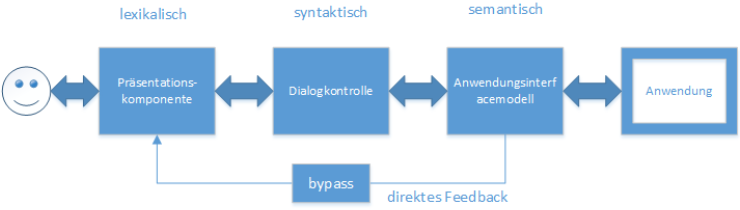
\includegraphics[scale=0.65]{Seeheim.PNG}

\subsection{Interaktionstechniken}
\begin{itemize}
\item \textbf{Menüs:} funktionieren z.B. auch rein text-basiert, sollten nicht mehr als $7\pm 2$ Verschachtelungen enthalten, "Breadcrumbs " zur Orientierung (z.B. Auswahl $\mid$ Auszahlung $\mid$ Betrag) 
\item \textbf{Frage/Antwort:} z.B. Abfragesprache wie SQL (in Menüs z.B. bei Online Registrirungen: Frage Bundesland, Antwort Sachsen; Frage PLZ...); Alexa, Siri, können aber nicht immer hilfreich antworten
\item \textbf{GUIs mit WIMP} = Windows Icons Menus Pointer ($\Rightarrow$ Fenster ermöglichen parallele Bearbeitung von Aufgaben)
\item \textbf{Formular/Dialog:} modale Dialoge erzwingen Abschluss des Dialogschritts (z.B. Druckerfenster); nichtmodale Dialoge erlauben parallele Bearbeitung von Aufgaben (z.B. Rechtschreibprüfung)
\item \textbf{Drag \& Drop:} z.B. für Fensterverwaltung und verschieben von Dateien
\item \textbf{3D Interaktion:} VR/AR, Motion Tracking, Smarphone GPS
\item Kommandozeile, Zeigen und Gesten, Multitouch 
\end{itemize}
\subsection{Anforderungsanalyse}
\begin{itemize}
\item eine Methode um kleinere Interaktionsschritte festzulegen ist \textbf{Card Sorting:} es wird ermittelt wie Benutzer Dinge benennen, gruppieren und die Gruppen benennen \\\\\\\\\\\\\\\\\\\\\\

\item unterschieden wird zwischen Mindestanforderungen und Zusatzfunktionen
\item \textbf{geschlossenes Card Sorting} = vorgegebene Gruppen (Nachteil: weniger Entscheidungsfreiheit für Benutzer) , \textbf{offenes Card Sorting} = ohne vorgegebenen Gruppen (Nachteil: schwierigere Auswertung (oft manuell))
\item unterschieden werden muss zwischen Anfoderung und Umsetzung: nicht "App braucht Play/Pause Knopf" sondern App hat Anforderung: Lied starten/stoppen, mögliche Umsetzung: Button
\item \textbf{Ethische Fragen} Werden die Daten anonym oder zumindest pseudonymisiert gespeichert? Können/Sollen z.B. behinderte Menschen oder Kinder teilnehmen? Haben Probanden Einverständnis und Freiwilligkeit erklärt, kennen sie den Zweck der Studie?
\end{itemize}
\subsection{Usability Engineering}
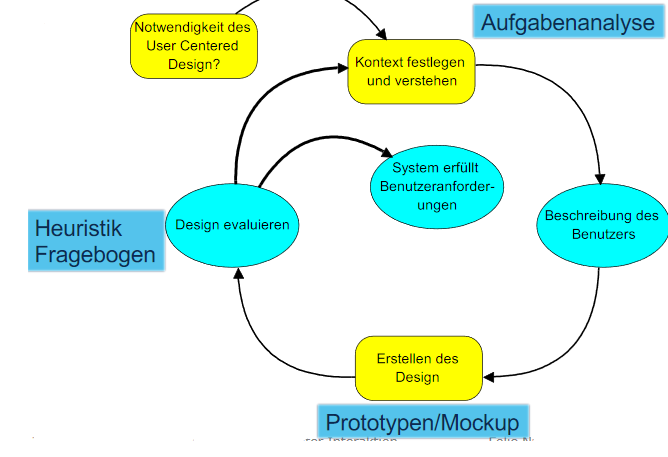
\includegraphics[scale=0.53]{UCD.PNG}
\begin{itemize}
\item wer ist Zielgruppe (expertise/eingeschränkt...)?, was ist der Nutzungskontext (online/offline, abgelenkt/konzentriert...)? welche Anforderungen ergeben sich daraus? wie setzt man diese um?
\item \textbf{Lo-Fi Prototypen} = Low Fidelity d.h. Skizzen, Storyboard, Wireframe (Gittermodell von z.B. Website, halt alles ohne Schriftart, Farben, Bildern), Papier (auch für haptische Oberflächen wie Braille), \textbf{Middle}: Mock-ups (Programm mit Papier und Pappe basteln), Wizard-of-Oz (Interaktion wird durch Menschen "hinter der Bühne" nachgebildet)
\item \textbf{Hi-Fi Prototypen} = High Fidelity d.h. Powerpoint, HTML, Programm grob entwickeln so dass Interaktionstechniken implementiert sind
\item Prototpyen verzichten oft auf optimale Effizienz und Zuverlässigkeit, sie haben oft Pseudodaten, vereinfachte Algorithmen, nur eine Zielplatform
\item \textbf{Effektivität} (von Effekt): tut es das was es soll? \textbf{Effizienz}: ist es Ressourcensparen? (auch nicht nur bzgl. Zeit); \textbf{Zufriedenstellung}
\end{itemize}


\section{Evalutaion}
\begin{itemize}
\item = Bewertung eines interaktiven Systems(von Experten oder Benutzer)
\item Ziel: Feststellung der Qualität der Benutzungsoberfläche
\item Qualitätsmerkmale: Effizienz(in angemessener Zeit), Effektivität(es funktioniert), Zufriedenehit
\item Methoden: Benutzer einzeln Befragen; Benutzer mit Fragebogen befragen
\item Heuristik nach Nievergelt: Wo bin ich?, Was kann ich tun?, Wie kam ich hierhin?, Wo kann ich hin?
\subsection{Heuristik}
\item = Verfahren, um Probleme zu lösen bei begrenztem Wissen und wenig Zeit
\item Heuristik zur Barrierefreiheit: \textbf{Wahrnehmbarkeit}, Bedienbarkeit, Verstehbarkeit, Robustheit
\item Barrierefreiheit: \textbf{Umfang}, in dem Produkte, Systeme,... durch Menschen mit weitesten Benutzererfordernissen genutzt werden können um Ziele zu erreichen
\item Figur-Grund-Wahrnehmung(selektive Interpretation und visuelle Unterscheidung) wird beeinflusst durch Wahrnehmung des Farbkontrasts
\subsection{Farbe}
\item Zäpfchen reagiern auf untersch. Wellenlängen (R,G,B), Stäbchen reagiern bei wenig Licht (schwarzweiß)
\item Farbkontraste: Wahrnehmung beeinflusst durch \textbf{Farbton}, \textbf{Helligkei}t, \textbf{Sättigung}; Definition von Kontrasten in Farbmodelle
\item RGB Farbmodell: rot, grün, blau; sRGB-Intervall[0,1]; 8bit-Intervall[0,255] oder in hex[000000,FFFFFF]; $R_{sRGB}=\frac{R_{8bit}}{255}$ entwickelt für \textbf{additives} Farbmodell(Röhrenmonitore); Umrechnung in anderen Farbraum für andere Technologien(LED, DLP)
\item Der Farbkontrast von zwei Farben ist dann ausreichend, wenn ihr Helligkeitswert das Verhältnis von t=3 (empirische Festlegung) oder besser aufweist t=$\frac{L_1+0,05}{L_2+0,05}$; 
\begin{itemize}
\item t=4,5 für normale und kleine Schrift (14 pt) für Level AA nach WCAG 2.0
\item t=3 für große oder fette Schrift (18pt bzw. 14 pt fett) für Level AA...
\item t= 7 für normale und kleine Schrift (14 pt) für Level AAA nach WCAG 2.0
\end{itemize}
\item Farbraum: zeigt welche Farben ausgenutzt werden können; für sRGB Weiß[0.3127,0.3290] 
\item Farbkontraste: Berechnung der Luminanz im sRGB Farbraum
\subsection{Evaluation mit Benutzern}
\item Methoden: Gebrauchstauglichkeit (Design, Äußere Benutzung, Zeit-/Fehlermessung), Benutzerstudien (beobachten/analysieren, der Ausführungen der Benutzer), Benchmarking(Kriterien: Objektivität, Validität, Reliabilität[Test geeignet für Prüfkriterium?]
\item Messgrößen(objektiv): Aufzeichnungen, Graphen, Zählungen(quantitiv, thematisch), Muster erkennen(qualitativ)
\item Diagramme berichten über Daten und erfinden keine zusätzlichen Daten (Punkte nicht verbinden, wenn keine Zwischenwerte existieren)
\item deskriptive Statistik: \textbf{Boxplot} zur Visualisierung(Minimum, 1.Quartil, Median(Zentralwert der Messdaten), 3.Quartil, Maximum)
\subsection{Fragebogen}
\item Hypothesen formulieren, Variablen und Merkmale dieser klären, zu erhebende Messwerte klären \item Anfangs allgemeine Fragen zur Person usw.; offene Fragen vorteilhaft aber schwer auszuwerten; negierte Aussagen zur Lügenerkennung, klare Aussagen, keine doppelte Verneinung
\item Likert Skala: bestehend aus bipolaren Behauptungen, Rating(Skala 1-5 als optimal erwiesen, da Mitttelwert existiert)
\item Aussagekräftigkeit: mehr als 80\% stimmen völlig zu(Ceiling-Effekt), mehr als 80\% lehnen ab(Floor-Effekt) 
\item erfüllen Gütekriterien: \textbf{Objektivität} (Ergebnisse unabhängig von Versuchsleiter), \textbf{Reliabilität} (gleiche Ergebnisse für denselben Gegenstand), \textbf{Validität} (misst was er messen soll)
\item NASA Task Load Index(TLX): Bestimmung des kognitiven Workload (mentale belastung); erhebung nach ausführung der Aufgabe
\item TLX Fragenkatalog: ermittelt subjektive mentale Belastung (workload) bei Bearbeitung einer Aufgabe oder im Umgang mit einem System 
\begin{itemize}
\item Mental Demand (MD): How mentally demanding was the task?
\item Physical Demand (PD): How physically demanding was the task?
\item Temporal Demand (TD): How hurried or rushed was the pace of the task?
\item Performance (OP): How successful were you in accomplishing what you were asked to do?
\item Effort (EF): How hard did you have to work to accomplish your level of performance?
\item Frustration (FR): How insecure, discouraged, irritated, stressed, and annoyed were you?
\end{itemize}   
\item anschließend Gewichtung der Fragen und Asuwertung; TLX kein perfektes System
\end{itemize}


\section{Text}
\subsection{Formeln und Umrechnungen}
\begin{itemize}
\item \textbf{Entropie} $H=-\sum_{i} p_{i}\cdot$ log$_{2}(p_{i})$ (durchschnittlicher Informationsgehalt)
\item \textbf{mittlere Wortlänge} $L=\sum _{i} p_{i}\cdot N_{i}$
\item \textbf{Redundanz} $R=L-H$, wobei $H\leq L$ (trägt nicht direkt zu  zu Information bei; nützlich z.B. für Fehlerkorrektur)
\item Basiseinheit bit, 8 bit $= 1$ byte, 1024 byte $=1$ Kib, 1024 Kib $=$ 1 Mib etc.
\end{itemize}
\subsection{Kodierungsverfahren}
\begin{itemize}
\item mit $n$ bit können $2^{n}$ zeichen codiert werden (dabei ist aber nich automatisch Fano-Bedingung erfüllt)
\item \textbf{Fano Bedingung} (auch Präfixeigenschaft): kein Zeichen bildet den Anfang eines anderen Zeichens\\ (z.B. Morse Code N$=-\bullet$, C$=-\bullet-\bullet \Rightarrow$ Fano Bedingung nicht erfüllt)
\item \textbf{Fano Codierung:} "WSKn absteigend sortieren, dann immer in 2 Gruppen teilen"; siehe C-Programm
\item \textbf{Huffman Codierung:} "immer letzten beiden WSKn zusammenfassen, Codebaum erstellen" \\ siehe people.ok.ubc.ca/ylucet/DS/Huffman.html\\ sind WSKn gegeben dann z.B. für (Zeichen X mit WSK $\frac{65}{100}$) in Python Konsole eingeben: print(65*”X”)
\item Es gilt: Huffman ist \textbf{effizienter}, Fano höchstens genau so effizient! (messbar über R und L)
\item \textbf{Zweck}: Verschlüsselung, Redundanzvermeidung, Digitalisierung analoger Signale, Schutz etc.
\end{itemize}
\subsection{Zeichensatz}
\begin{itemize}
\item \textbf{Braille:} gibt es für fast alle Sprache, allerdings hoher Pflatzbedarf
\item \textbf{ASCII:} 128 Zeichen mit je 7 bit, Zeichen 0 bis 31 sind Steuerzeichen (wie unser Enter...); Darstellung oft als Hexadezimal
\item \textbf{Latin:} 8 bit Zeichensatz, erste 128 Zeichen identisch zu ASCII, es gibt verschiedene Varianten je nach Region (Latin-6 Nordisch, Latin-5 türkisch etc.)
\item \textbf{Unicode:} internationaler Standard, Anzahl codierbarer Zeichen variiert nach Version,in diesem Dokument z.B. UTF-8 $\Rightarrow$ "A" wird zb als 41 (Hex) codiert (detaillierte Codierungsregeln siehe Folie 20 Medien-Text)
\end{itemize}
\subsection{Schrift}
\begin{itemize}
\item Schriftgößeeinheiten für DTP Standard (Achtung: bei anderen Standards ist z.B. 1 point anders definiert): 1 pica $=12$ points $=12 \cdot 0,352\overline{7}$ mm 
\item \textbf{Serifen} (die kleinen "Verzierungen" an den Enden aller Buchstaben) helfen bei Lesbarkeit 
\item bei \textbf{Rasterschrift} bestehen Zeichen aus Pixeln
\item bei \textbf{Vektorschrift} bestehen Zeichen aus Kurven ($\Rightarrow$ wird beim reinzoomen nicht verpixelt)
\end{itemize}
\subsection{Formatierung}
\begin{itemize}
\item \textbf{Kerning/Unterschneidung:} Abstand zwischen zwei Buchstaben wird vom Textverarbeitungsprogramm manchmal gesondert angepasst, z.B. bei parallelen Diagonalen bei Text "AV", Diagonalen vom A und V werden näher aneinander gerückt
\item neben \textbf{Blocksatz} gibt es \textbf{Flattersatz} (Links-/Rechtsbündig) und \textbf{Mittelachsensatz} ("zentriert")
\end{itemize}
\subsection{Formate und Software}
\begin{itemize}
\item eine Eigenschaft von Editoren ist \textbf{WYSIWYG} ("what you see is what you get"; z.B. bei Word, z.B. nicht bei Latex)
\item \textbf{Rich-Text:} z.B. in MS Word; nicht programmierbar
\item \textbf{HTML:} Integration verschiedenster Medien möglich, erweiterbar durch Plugins, "Aussehen" eines Dokumentes wird getrennt vom allen anderen Sachen im "Style sheet" festgelegt, Dynamisch durch Scripting 
\item \textbf{Latex:} programmierbar, gut für Formeln, Latex ist nur die Interface-Sprache für das Textsatzsystem TeX 
\item \textbf{PDF:} kann nur mit spezieller Software bearbeitet werden, Integration verschiedenster Medien möglich, Layout-treu ("wird immer gleich wiedergegeben")
\end{itemize}


\section{XML(eXtensible Mark-up Language)}
\begin{itemize}
\item Medien in Dokumenten definieren sich durch \textbf{Inhalt} (Semantik), \textbf{Struktur} (Syntax) und \textbf{Präsentation} (lexikalische Information)
\item Für Arbeiten mit HTML bedient man sich der Sprache, Werkzeugen und Arbeitsmethoden (Layouten o. ä.). HTML basiert auf XML, das als \textbf{Metasprache} Text beschreibt und strukturiert (Baumstruktur). 
\item Dokumente bestehen aus Tags\\
\lstinline|<person>Der Bart</person>| oder für leere Elemente \lstinline|<br/>|; Elementname (person) legt das Tag als Ganzes fest. Metazeichen von XML sind entsprechend zunächst \lstinline|<, > und /|.
\item Elemente können Elemente enthalten (Schachtelung); Elemente können Text enthalten; Groß- und Kleinschreibung bei Elementnamen beachten; Das öffnende Tag muss genauso lauten wie das Schließende
\item In XML-Dokumenten immer XML-Deklaration am Dokumentenbeginn: \lstinline|<?xml version="1.0"?>|. Folgen kann dann ein \textbf{Stylesheet} und eine \textbf{DTD} sowie die \textbf{Daten}.
\item \textbf{Wohlgeformtes} XML ist syntaktisch korrekt (s. o., mit korrekten Schachtelungen, richtig verwendeten Metazeichen, genau ein Wurzelelement, etc); \textbf{Valides} XML erfüllt die angegebene DTD; mittels Parser prüfbar
\item \textbf{Sytntaxdiagramme}: Es gibt ein (nichtterminales) Startsymbol; Symbole in Kreisen sind terminal; Symbole in (abgerundeten) Rechtecken sind nichtterminal, beziehen sich auf andere Symbole; Ausdruck ist "wohlgeformt", wenn ein Durchlauf durch die Diagramme möglich ist
\item \textbf{Wichtige Begriffe}: Elemente, Knoten (Tags), Vorgänger, Nachfolger, Nachbarknoten, Wurzel, Attribute, Text
\item hierarchischer Aufbau in XML Bäumen, Reihenfolge wichitg
\item XML-Tags müssen mit Buchstaben oder '\_` anfangen, danach alphanum. Zeichen mgl.; dürfen keine Metazeichen (<>"/' etc.) oder Leerzeichen enthalten
\item \textbf{Entitäten} in XML "definieren Kurzformen für Standardtext oder Sonderzeichen" z. B. \lstinline|&lt; &gt; &quot;| für das \lstinline|< > "|-Zeichen; (\lstinline|&...;|) sind "Fluchtsymbole" in XML. Dadurch können alle Metazeichen in XML auch verwendet werden (\lstinline|&| wird durch \lstinline|&amp;| gesetzt)
\item \lstinline|<[!CDATA[<svg></svg>]]| ermöglicht Textabschnitt ohne Fluchtsymbole(alle Metazeichen zulässig außer ]])
\item In der XML-Deklaration kann \textbf{Attribut} \lstinline|encoding="iso8859-1"| und \lstinline|standalone="no"| (gibt an, dass die DTD im Dokument selbst drin ist) verwendet werden
\item Kommentare: \lstinline|<!-- Kommentar -->|
\item Element \textbf{Attribute}: ist ein Paar \textit{"Attributname=Attributwert"}, kann an Elementname angehängt werden; mit Anführungszeichen begrenzt; mehrere pro Element möglich
\item \textbf{Processing instructions} weisen auf Verarbeitungsschritte hin;
\subsection{DTD}
\item DTD ist selbst kein XML, definiert Struktur, gibt Aufbau der XML-Daten mit Reglen(legt Reihenfolge der Elemente fest) an, beschreiben nicht die Semantik der Daten
\item Beispieldefinition:
\begin{lstlisting}
<!DOCTYPE person [
<!ELEMENT person(fname,profession*)>
<!ELEMENT profession(#PCDATA)>
<!ELEMENT fname(#PCDATA)>
]>
<person>
<fname>Tim</fname>
<profession>Troll</profession>
<profession>Toll</profession>
</person>
\end{lstlisting}
\item \lstinline|<!ELEMENT (...)>| definiert ein Element und in Klammern die erwarteten Kindelemente, in fester Reihenfolge. Man kann \textbf{\lstinline|?|} für ein-oder-keinmal anfügen, \textbf{\lstinline|*|} für beliebig oft (oder gar nich), \textbf{\lstinline|+|} für ein oder mehr; Alternativen möglich mit \lstinline{((a, b) | (c, d))}; \lstinline|#PCDATA| für beliebig viel normalen Text; EMPTY (statt der Kindelementliste $\Rightarrow$ besitzt keine) wenn Element immer leer sein soll; ANY für komplett egal
\item \textbf{Textzeichen mit Elementen mischen}: \lstinline{<!ELEMENT paragraph (#PCDATA | name |} \lstinline{ profession |footnote | emphasize | date)*>} (kann durch * beliebig oft permutiert werden)
\item \textbf{Attributtypen} sind z. B. CDATA (Text), ID (eindeutiger XML-Name), NMTOKEN (wohlgeformter XML-Name), IDREF (Name eines anderen im XML vorkommenden Elements[für eindeutige sichere Verknüpfungen]), IDREFS (Mehrere Namen von anderen XML-Tags im Dokument, getrennt durch Leerzeichen)
%\item \lstinline|<!ATTLIST img		source CDATA|\\
%\lstinline|#REQUIRED w CDATA #REQUIRED| gibt Attributliste für das img-Element an. 
\item \textbf{Attribute} für Elemente sind \#REQUIRED (muss vorhanden sein), \#FIXED (muss immer einen bestimmten Wert haben, der danach angegeben wird), \#IMPLIED (optional). Alternativ kann eine beliebige Zeichenkette geschrieben werden, die den Standardwert angibt.
\item \lstinline{<!ATTLIST name first CDATA #REQUIRED>} fügt Attribute(first) zu einem Element(name) hinzu
\item XML-Namen gehören einem Namensraum, d.h. einer Syntaxbeschreibung an; durch Präfix können identische Elemente (XML-Namen) verschiedener Namensräume unterschieden werden; Alle Elemente verschiedener DTDs müssen unterschieden werden; (wird bei Elementen durch allgemeingültiges Attribut xmlns deklariert) möglchkeit SVG oder HTML Code in XML zu integrieren
\item XML für Dokumente: Text Encoding Initiative(TEI) mit TDT für Theater o. ä. 
\item DocBook / OpenEBook: XML für Bücher wie Informatikbücher
\item MusicXML: zum Musikstücke digitaliseieren
\item DTDs können keine Zahlen oder Maximallängen vorgeben, keine Modularisierung, DTDs sind keine XML-Dokumente
\end{itemize}


\section{XSLT}
\begin{itemize}
\item Daten von der Präsentation trennen, Transformation von XML-Struktur in neue Struktur, Formatierung der neuen Struktur
\item Einbindung eines XSLT-Stylesheets:\\
\begin{lstlisting}
<?xml-stylesheet type="text/xsl"
href="helloworld.xsl"?>
<?xml version="1.0" encoding
="iso-8859-1"?>
<greeting>Hallo Welt!</greeting>
\end{lstlisting}
Beispiel des XSLT-Stylesheets:
\begin{lstlisting}
<xsl:stylesheet version="1.0"
xmlns:xsl="...">
<xsl:template match="/">
<html><head>
<title>Wort zum Tag
</title></head>
<body><p>
<xsl:value-of select="greeting"/>
</p></body></html>
</xsl:template>
</xsl:stylesheet>
\end{lstlisting}
\item Verarbeitung basiert auf Templates, auch ECMA-Script möglich
\item \lstinline|<xsl:apply-templates>| führt die Templates, bei Angabe von select nur auf entsprechende Elemente, \lstinline|<xsl:value-of select="elemtname">| holt den Wert eines XML-Tags und fügt ihn an dieser Stelle ins Dokument ein, \lstinline|<xsl:for-each select="a">| gibt für jedes folgende Element den definierten Text aus, \lstinline|<xsl:template match="people">| gibt für alle people-Elemente im XML den definierten Text aus
\item Mit dem Attribut mode für apply-templates und template kann Status definiert werden, z. B.
\item \lstinline|<xsl:variable name="width" select="50"/>| legt Variable width=50 fest
\item \lstinline|<xsl:if test="position()=1"></xsl>|
\item \lstinline|<xsl:for-each select="book"></xsl>|
\item \lstinline|<xsl:sort select="author"></xsl>|
\item XPATH wird in XSLT benutzt, um Tags anzusprechen (match-Attribut). \/ ist die Wurzel, Tagnamen werden als Nachfolger interpretiert, der zugehörige Tag eines Attributes kann mit @born angesprochen werden
\item In XPATH kann gerechnet werden (div, +, - , *, mod, position(), first(), count(), round(), substring())
\end{itemize}


\section{Bild}
\subsection{SVG}
\begin{itemize}
\item EncapsulatedPostScript, Bildinformationen in speziellem Code, programmierbar, keine Alphakanäle, nur PostScript-Geräte
\item Scalable Vektor Graphics (SVG) in XML für Bilder, Text, Animation, Formen (bspw. mit Inkscape malbar)
\item Pfade: \lstinline|<path d=""></path>|, Möglich anzugeben: M x y (Zeichenstift ohne zu zeichnen bewegen), L x y (Linie zum Ziel malen), Q x1 y1 x2 y2 (Quadratische Bezier-Kurve), C x1 y1 x2 y2 x3 y3 (Kubische Bezier-Kurve), Z (Pfad schließen), H x (Horizontale Linie), V y (Vertikale Linie), A ??? (Ellipsenbogen), S x y (Quadratische Bezierkurve fortsetzen, vorherigen Kontrollpunkt spiegeln) - Groß geschriebenes Zeichen steht für absolute, kleines für relative Koordinaten. Pfade beginngen immer mit moveto (M) und können mit Z enden.
\item Primitive: circle-Element mit Attributen cx, cy und r (CenterX und CenterY), ellipse mit cx, cy, rx und ry, rect mit x, y, width, height, line mit x, y, width, height, polygon / polyline mit points (x1 y1 x2 y2...)
\item Text: text-Element mit x, y, size
\item Image: image-Element mit x, y, width, height, xlink:href
\item Einfärben von Formen mit fill-Attribut und einer Farbe in Hex (\#FF0000 z. B.) oder Name.
\item Rand malen mit stroke-Attribut (enthält Farbcode) und stroke-width-Attribut (Randbreite in Pixeln)
\item transform-Attribut gibt Rotation, Transformation, Skalierung oder Stauchung an: z. B. "translate(20, 150) scale(0.5) rotate(30,255,230) skewX(25) skewY(25)" - Bei Rotate dienen der zweite und dritte Parameter dabei als Rotationszentrum
\item Clipping: Beschränken eines zu zeichnenden Elements auf den Bereich, den ein anderes Element definiert
\item Filter in SVG: "Fotorealismus" durch Unschärfe, gezielte Einbringung von Bildstörungen o. ä.
\item Blurring: Unschärfefilter
\item Events in SVG mit JavaScript definiern (svg onload-Event, onclick-Event etc.)
\item \begin{lstlisting}
<ellipse id="elli" cx="100" cy="100"
rx="48" ry="90" style="fill:green;"
/><animate xlink:href="#elli"
attributeType="XML" attributeName="rx"
begin="0s" dur="6s" from="48"
to="198" fill="freeze" />
\end{lstlisting}
\item In \lstinline|<defs>...</defs>| können SVG-Elemente definiert werden, die nicht gezeichnet werden, sondern mit \lstinline|<use xlink:href="#id">| später wieder benutzt werden
\end{itemize}
\subsection{Licht}
\begin{itemize}
\item Licht ist eine elektromagnetische, transversale Welle (schwingt parallel zur Ausbreitungsrichtung)
\item Lichtgeschwindigkeit im Vakuum $c = 299792458 \frac{km}{s}$ ist vom Medium, in dem sich das Licht bewegt, abhängig (meist Luft), $c = \lambda * f$ (f: Frequenz des Lichts, $\lambda$: Mediumskonstante)
\item Frequenz ist Maß für Energie $E = hf = \frac{h c}{\lambda}$ (h ist das Planksche Wirkungsquantum mit ca. $h = 6.63 * 10^{-34} Js$), d. h. je höher die Frequenz, desto energiereicher ist das Licht.
\item Frequenz des sichtbaren Lichts beträgt ca. 400 nm - 780 nm, davor liegen die Frequenzbereiche von UV-Licht, Röntgen- und Gammastrahlung, darüber die von infrarotem Licht, UKW-Radio etc
\item Je höher die Frequenz, desto geringer die Wellenlänge (antiproportional)
\item Lichtemission: Durch Gasentladung (z. B. Xenon Lampen), Photolumineszens (Phosphor "wandelt" einfallendes Licht in andere Wellenlänge um)
\item Chemische Reaktion: Verbrennung (Flamme strahlt Licht)
\item Phosphor: Elektronenbeschuss bringt Phosphor zum Leuchten
\item Absorption: Bspw. beim Durchlaufen einer farbigen Folie wird ein Teil des Lichtspektrums absorbiert
\item Reflexion: Ein Teil des Lichts wird beim Auftreffen auf eine Oberfläche reflektiert
\item Additive Farbmischung: Überlagerung von Licht mehrerer Emissionsquellen, Spektren werden addiert
\item Subtraktive Farbmischung: Einfallendes Licht fällt auf Filter (Absorption / Reflexion) ("Multiplikation mit Filterfunktion")
\item Gedruckte Farben erscheinen je nach Beleuchtung unterschiedlich (z. B. Geld wird rötlich bei roter Beleuchtung...) 
\item Farbtemperatur in Kelvin: "Wärme" des Lichtes, je höher desto weißer - Glühlampe ca. 2800K, 6500K: Tageslicht
\item Mensch "sieht" Lichtintensität, visuelle Wirkung, Konstrast, Formen, Bewegung
\item Sehen beeinflusst Wachsamkeit, Wohlbefinden, innere Uhr [...]
\item Spezielle Rezeptoren, spezieller Nervenpfad im Hirn
\item Retina im Auge mit Photorezeptoren besetzt, Fovea im Zentrum des Sehfeldes, "blinder Fleck" des Auges ca. 1,75mm im Durchmesser (Gehirn "vervollständigt" das Bild)
\item Farbwahrnehmung in der Retina erfolgt durch Zapfen und Stäbchen (Zapfen: Farbwahrnehmung, Stäbchen: Schwarz/Weiß)
\end{itemize}
\subsection{Farbmodelle}
\begin{itemize}
\item RGB-Farbraum: 256 Farbstufen pro Rot, Grün und Blau, also ca. 16 Millionen Farben
\item CIE 1932: xyz-Kanäle, y: Wahrgenommene Helligkeit, x: rot/grün, z: blau/gelb-Unterschied
\item Farbwahrnehmung: Helligkeit (Luminance), Farbton und Sättigung (Saturation) hauptsächlich
\item Hirn teilt wahrgenommene Farben in weiß, grau, schwarz und verschiedene Farben
\item 128 Farbtöne (Hues), 130 Farbsättigungen (Saturation Levels), 16 (blau) - 26 (gelbe) Helligkeitswerte, also ca. 7 Millionen wahrnehmbare Farbnuancen
\item Farben in Text: Hervorhebung, sparsam (auffällige) Farben einsetzen
\item Räumliches Sehen durch Augenabstand (Fusion, Disparität) zum Erkennen von relativer Größe, Perspektive, Beleuchtung
\item Hirn bildet 3D-Modell (Fusion): Unterdrückung unvereinbarer Regionen, bei Überlagerung wechselt unvereinbares linkes / rechts Bild
\item Räumliches Sehen: Fokus (Raumpunkt, auf den die Augen fokussiert sind), Retinale Position (relative Position zur optischen Achse), Mentales Auge: Fusion kombiniert Information
\item Disparität: Unterschied von fusionierten Punkten kann zur Berechnung der relativen Position benutzt werden
\item Munsell Farbsystem (Farbton hue, Helligkeit value, Sättigung chroma)
\item HLS Farbsystem (Hue, Luminance, Saturation)
\item CMY - Farbraum (Cyan, Magenta, Yellow)- $(r, g, b) = (1, 1, 1) - (c, m, y)$
\item CMYK - CMY mit Schwarz, damit Schwarz nicht aus Farbe gemischt werden muss (für Drucker toll)
\item YUV - Y: Helligkeit (s / w), U, V: Farbbalance
\item $YC_bC_r$ - Y: Helligkeit, b: Blau, r: Rot
\end{itemize}
\subsection{Digitale Bilder}
Digitale Bilder bestehen aus Pixeln ($w * h$), die pro Pixel meist 8 - 32 bit Farbinfos beinhalten (Farbtiefe des Bildes) (ab 24 bit: TrueColor)
\begin{itemize}
\item Indizierte Farbformate: Zu Beginn des Bildes Farbtabelle, danach wird jede Farbe mit einem Index auf die Farbtabelle angegeben (sinnvoll bei wenigen verwendeten Farben)
\item Chroma Subsampling bei YUV und $YC_bC_r$ (4 : 2 : 2): Halbe Auflösung für g/b (U) und r/gr (V)-Kanäle
\item Alphakanal: Transparenzangabe
\item Auflösung des Auges: $\phi$ minimaler Sehwinkel, bei dem 2 Linien im Abstand $s$ erkannt werden, $s = 2a * tan(\frac{\phi}{2})$
\item dpi / ppi: dots per inch / pixels per inch (Pixel pro Zoll, $1 in = ~2,54cm$)
\item Monitor ca. 95 ppi, Laserdrucker ca. 1400 dpi
\end{itemize}
\subsection{Digitale Bildformate}
\begin{itemize}
\item Histogramm: Gibt Verteilung der Graustufen von 0-1 des Schwarzwertes an
\item Bildfilter: Beispielsweise Weichzeichner (lineare Mittelwertbildung aus Nachbarn um einen Pixel herum)
\item GIF, Graphics Interchange Format: Animierbares farbindiziertes Bildformat mit 256 Farbstufen, kein Alphakanal, verlustbehaftete Kompression
\item PNG: Portable Network Graphics: verlustfreie Kompression als GIF, Alphakanäle, freies Format, keine Animation, nicht für Fotos geeignet (verlustfreie Kompression zu schwach), Interlacing (Zunächst werden nur einige Zeilen des Bildes übertragen und dadurch eine Vorschau möglich, bevor das gnaze Bild übertragen ist)
\item JPEG (Joints Photographic Experts Group): Verlustbehaftete Kompression u. a. mit Huffmann-Kodierung, Bildung von 8x8-Blöcken - führt zu Blockbildung, JPEG-2000 als Nachfolger mit geringerer Artefaktbildung - Farbraumumrechnung in YUV, Tiefpassfilterung \& Unterabtastung der Farbdifferenzsignale U, V (verlustbehaftet 4 : 2 : 2, s.o.), Quantisierung, Umsortierung, Huffmann-Kodierung. Gut geeignet für Fotos, nicht gut für alles andere (Diagramme etc)
\item JPEG2000 basiert auf XML - ermöglicht Rechtemanagment, verschieden starke Komprimierung in verschiedenen Bildteilen, Interlacing-Support
\item TIF - Tagged Image Format: mehrere Farbräume wie RGB, LAB, verlustfreie Komprimierung mit LZW, schwache Komprimierung, können viele Browser nicht
\item PSD - Adobe Photoshop, Kanäle, Bearbeitungsschritte, Text wird nicht gerastert, kann von vielen Programmen nicht gelesen werden
\end{itemize}
\subsection{Vektorgrafik}
\begin{itemize}
\item Vektorgrafik - Beschreibung des Bildes mittels Formen wie Rechtecken und nicht durch Pixel (Bsp.: SVG)
\item Transformationen (Rotation, Translation, Skalierung, Scherung) können mittels der Multiplikation des alten Vektors mit einer Matrix und der Addition eines neuen Vektors ausgedrückt werden.
$\begin{pmatrix}
x' \\ y'
\end{pmatrix} = \begin{pmatrix}
a & b \\ c & d 
\end{pmatrix}\begin{pmatrix}
x \\ y
\end{pmatrix} + \begin{pmatrix}
e \\ f
\end{pmatrix}$
\item Translation: $\begin{pmatrix}
x' \\ y'
\end{pmatrix} = \begin{pmatrix}
1 & 0 \\ 0 & 1 
\end{pmatrix}\begin{pmatrix}
x \\ y
\end{pmatrix} + \begin{pmatrix}
\Delta x \\ \Delta y
\end{pmatrix}$
\item Rotation: $\begin{pmatrix}
x' \\ y'
\end{pmatrix} = \begin{pmatrix}
\cos \alpha & -\sin \beta \\ \sin \alpha & \cos \alpha 
\end{pmatrix}\begin{pmatrix}
x \\ y
\end{pmatrix} + \begin{pmatrix}
0 \\ 0
\end{pmatrix}$
\item Scherung: $\begin{pmatrix}
x' \\ y'
\end{pmatrix} = \begin{pmatrix}
1 & s \\ 0 & 1
\end{pmatrix}\begin{pmatrix}
x \\ y
\end{pmatrix} + \begin{pmatrix}
0 \\ 0
\end{pmatrix}$
\item Skalierung: $\begin{pmatrix} x' \\ y' \end{pmatrix} = \begin{pmatrix}
a & 0 \\ 0 & b
\end{pmatrix}
\begin{pmatrix} x \\ y \end{pmatrix} + \begin{pmatrix}
0 \\ 0
\end{pmatrix}$
\item Bezierkurven dritten Grades / kubische Kurven: Kurven nach dem Format:
$\begin{pmatrix} x(t) \\ y(t) \end{pmatrix} = (1-t)^3 \begin{pmatrix} x_0 \\ y_0 \end{pmatrix} + 3t(1 - t)^2 \begin{pmatrix} x_1 \\ y_1 \end{pmatrix} + 3t^2(1 - t) \begin{pmatrix} x_2 \\ y_2 \end{pmatrix} + t^3
\begin{pmatrix} x_3 \\ y_3 \end{pmatrix}$
Dabei sind $\begin{pmatrix} x_0 \\ y_0 \end{pmatrix}$ und $\begin{pmatrix} x_3 \\ y_3 \end{pmatrix}$ die Start- bzw. Endpunkte der Kurve und $\begin{pmatrix} x_1 \\ y_1 \end{pmatrix}$ sowie $\begin{pmatrix} x_2 \\ y_2 \end{pmatrix}$ definieren die Tangenten an diesen Punkten.
\item de Casteljau-Schema: $t = \frac{1}{4}$
\item TrueType-Fonts: Die Kontur von Zeichen werden durch Bezierkurven beschrieben, wird dann gefüllt
\item Meta Font (\LaTeX): Glyphenkontur wird durch interpolierende Kurve beschrieben
\item Gruppierung von einzelnen Formen, damit Transformation auf alle Elemente angewendet werden können
\item Tiefe: Definierung einer Koordinate z, damit die Überlagerungsreihenfolge bei überlappenden Formen definiert werden kann
\item Rasterisierung: Übersetzung von Vektorgrafik in Pixelgrafik (durch Test jedes Bildpunkts, ob er in einer Form liegt oder durch zeilenweises Abtasten [Sweepline], oder durch Abtasten jeder Form und Setzen der ausgefüllten Pixel)
\item Dropouts (bei TrueType-Fonts): Nur halb ausgefüllte Pixel werden falsch als nicht gegeben gesetzt, daher setzen TrueType-Abtaster einen Pixel zwischen zwei anderen Pixeln auch dann, wenn zwischen diesen Pixeln zwei Konturlinien der Glyphe liegen (aber nur dann, wenn beide Konturen in beide Richtungen fortgesetzt werden)
\end{itemize}
\section{Wahrnehmung}
\begin{itemize}
\item Motivation: Notwendige Daten an menschliche Warnehmung anpassen, um Platz zu sparen (z. B. nicht wahrnehmbare Töne bei Audio)
\item Ergonomisch physische Dinge gestalten, Gestaltung von Benutzerschnittstellen, Layout etc. auf Menschen optimieren
\item $Reiz \rightarrow Sensor (analog) \rightarrow Filter \rightarrow Quantisierung (Digitalisierung) \rightarrow Filter (digital) \rightarrow Kompression \rightarrow Codierung \rightarrow Speichermedium$
\item $Speichermedium \rightarrow Decodierung \rightarrow Dekompression \rightarrow Filter (digital) \rightarrow Rekonstruktion \rightarrow Filter (analog) \rightarrow Display (analog) \rightarrow Reiz (beim Mensch)$
\item Wie funktioniert Reiz? Wie werden Reize beim Menschen wahrgenommen (Visuell, Akustisch, Haptisch, Gustorisch / Geschmack, Olfaktorisch / Geruch), Multimedial: Sprache und Deixis, Multimodal: Gedächtnisleistungen. Wie stark wird welcher Reiz wahrgenommen? Wie gleicht man produzierten Reiz mit echtem Reiz ab?
\item "Wahrnehmung ist der Prozess, durch den Lebewesen Kenntnisse über ihre Umgebung und über sich selbst in Beziehung zur Umgebung gewinnen. Sie ist der Anfang allen Wissens."
\item Reize / Wahrnehmung / Neuronale Prozesse
\item Funktionale Physiologie: Erkenntnisse durch Patienten mit verletzten Gehirnen, elektrische Störungen von außen, durch teilweise Einschläferung, mit Elektro-Enzephalographie, Magneto-Enzephalographie
\item Wahrnehmung ist relativ: Größe / Helligkeit 
\item Wahrnehmung der Länge erfolgt logarithmisch (bei längeren Strukturen müssen Unterschiede größer sein)
\item Wahrgenommene Skalen für Größe von Kreisen ist abhängig nach vom Radius
\item Spitze Winkel werden unter- und stumpfe Winkel überspitzt
\item Reizschwelle $R_0$: kleinster wahrnehmbarer Reiz (z. B. Helligkeit des dunkelsten, noch erkennbaren Sterns am Nachthimmel), quantitativs Maß (z. B. Pa beim Hören) 
\item Unterscheidungsschwelle $\Delta R$: kleinster Unterschied von einem Grundreiz (z. B. Helligkeitsdifferenz für einen Punkt, den man gerade noch auf einem grauen Hintergrund wahrnehmen kann), qualitatives Maß 
\item Messverfahren erfordern Wahrnehmung von Reizen: Methode konstanter Reize (Zufällige Wiedergabe von verschieden starken Reizen, der zu 50\% erkannte Reiz ist die Reizschwelle - sehr genau, langsam), Hterstellungsmethode (VP stellt den Reiz selbst ein - ungenau, schnell), Grenzmethode (Reiz erhöhen bis ihn VP erkennt - genau, langsam)
\item Empfindungsstärke $\Psi$, Intensität des Grundreizes $R$, Unterscheidungsschwelle $\Delta R$, $k$ von Sinnesmodalität abhängige Konstante
\item Webersches Gesetz: $\frac{\Delta R}{R} = k$
\item Weber-Fechnersches Gesetz: $\Psi(R) = c * ln \frac{R}{R_0}$
\item Quadriert man die Stärke des Grundreizes, dann verdoppelt sich die Empfindungsstärke
\item Stevensches Potenzgesetz: $\Psi(R) = c * (R - R_0)^n$. Entscheidend ist der Parameter $n$. Für Helligkeit gilt $n = 0.3$, für ein Gewicht $n = 1.5$, für die Länge einer Linie $n = 1.0$
\item Empfindungsstärken wie Lautstärke: Verwendung einer logarithmischen Einheit wie Dezibel (Weglassen von k)
\item Bel: Logarithmus des Quotienten zweier Leistungen $Pegel = lg \frac{R}{R_0}$, Dezibel: Zehntel eines Bels $Pegel = 10 * lg \frac{R}{R_0}$
\item Wahrnehmung: Extraktion elementarer Merkmale (Kanten, Farbe), Präattentive Verarbeitung (Erkennen elementarer Bestandteile), Attentive Verarbeitung (Konstruktion des Gesamten)
\item Wörter eines Textes werden nicht Buchstabe für Buchstabe wahrgenommen (Auge liest 6-8 Buchstaben und springt dann weiter), Hören funktioniert ähnlich
\item Gesetz der guten Gestalt / Prägnanz: Übergeordnetes Gesetz zur Wahrnehmung von Gegenständen, Zusammenführung von prägnanten Einzeleindrücken zu Gestalt
\item Gesetz von Figur und Grund: Figur wird als vor dem Hintegrund stehend wahrgenommen, Figur und Grund kann nicht gleichzeitig wahrgenommen werden
\item Gesetz der Gleichheit: Ähnliche Dinge erscheinen zu zusammengehörigen Gruppen geordnet
\item Gesetz der Nähe: Dinge, die sich nebeneinander befinden, erscheinen als zusammengehörig
\item Gesetz der Geschlossenheit: Von Linien umschlossene Gegenstände werden als zusammengehörig empfunden
\item Gesetz des weiterführenden oder gleichen Verlaufs: Bruchstücke reichen zum Bilden von Gestalten aus
\item Gesetz der Symetrie: Symetrische Gebilde werden als Figur wahrgenommen
\item Gesetz des gleichen Schicksals: Objekte, die sich mit gleicher Geschwindigkeit bewegen, werden als zusammengehörig empfunden
\item Gesetz der Erfahrung: Wiedererkennen von bestimmten Formen
\item Gestaltgesetze betreffen die präattentive Wahrnehmungsphase und finden vor allem z. B. bei der Interfacegestaltung Anwendung (Gestaltung von Icons, Bedienoberflächen)
\item Bei rivalisierenden präattentiven Prozessen kommt es zu Wahrnehmungstäuschungen, Linien werden gebogen
\item Geone: Dreidimensionale Grundformen werden präattentiv anhand der Kantenanordnung erkannt und dann attentiv zu einem Gegenstand wie einem Tisch zusammeninterpretert
\end{itemize}


\section{Internetz}
\begin{itemize}
\item \textbf{HTTP}: Protokoll zwischen Web-Server und Web-Client (Browser)
\item \textbf{URI}: Bezeichnung und Adressierung beliebiger Daten im Netz (z. B. http://www.wh2.tu-dresden.de)
\item \textbf{Hypertext}: "Nicht-lineares" Textmedium, verbindet Inhalte durch Hyperlinks (URI, entfernte URIs wie "http://google.de", "ftp://..." oder lokale URIs wie "mailto:", die an andere Programme auf dem Rechner gehen)
\item \textbf{Mark-Up-Sprachen}: Beschreibung von Text durch Text, bspw. HTML mit öffnenden Tags und schließenden Tags und Inhalt dazwischen
\end{itemize}
\subsection{HTML}
\begin{lstlisting}
<html><head><title>Hallo Welt</title>
</head><body><h1>Grosse Ueberschrift
</h1><a href="uri">Link</a></body></html>
\end{lstlisting}
\begin{itemize}
\item Attribute bspw. href mit Ziel-URI, align mit Ausrichtung o. ä.
\item \lstinline|<a>|-Elemente sind Anker, verlinkt wird per \lstinline|"#ziel"| und gesetzt per name-Attribut
\item Bilder mit
\lstinline|<img src="uri" alt="beschreibung"|
\lstinline|width="300" height="300">|
\item Listen mit ul (unordered list) und ol (ordered list)-Elementen, Einträge mit li (list item)-Elementen
\item Tabellen mit table, tr für Zeilen und td für Spalten.
\begin{lstlisting}
<table><tr><th>1</th><th>2</th></tr>
<td>A</td><td>b</td></tr></table>
\end{lstlisting}
\item div für allgemeine Blöcke
\end{itemize}
\subsection{Barrierefreiheit}
Barrieren für Behinderte auf Webseiten (Sehbehinderte, Farbenblinde, Gehörbehinderte, Motorisch behińderte, geistig behinderte)
\subsection{CSS}
Strikte Trennung zwischen Präsentation und Design, definierte Formate für XHTML-Tags. Text-Formatierung, Positionierung von Elementen, Rahmen und Leerräume, Hintergrund, Formatierung von Tabellen, CSS einbinden mit \lstinline|<style type="text/css"></style>| für direktes Reinschreiben von CSS, CSS-Datei im Head des HTML-Dokuments verlinken mittels \lstinline|<link rel="stylesheet"| \lstinline|type="text/css" href="datei.css">|. HTML-Elemente koennen auch mit style-Attribut und CSS-Angaben gestyled werden.\\
CSS besteht aus Selektoren für Elemente (mittels ID oder Klasse) und Style-Attributen. Bspw.: \lstinline|#foo { color: red; }| setzt die Schriftfarbe im Element mit der ID foo auf rot. Mögliche Styleattribute sind z. B. "font-family" (Arial, sans-serif), "font-weight" (bold).\\
\subsection{Positionierung}
Mit CSS werden Elemente nach dem Boxmodel layoutet, d. h. jedes Element bildet eine Box. CSS-Attribute für jedes Element sind z. B. "margin" (Außenrand um die Box des Elements, z. B. "5px"), "padding" (Innenabstand um den Boxrand), "border-width" (Randbreite), "border-color" (Randfarbe).
\subsection{Navigationstechniken}
Websiten sollten sets einwandfrei navigierbar sein (vor / zurück, Nutzer muss sich zurechtfinden können). Bspw. durch Setzen von Navigationsleisten, Suchmaschinen etc.
\subsection{Karten in HTML}
Map-Element definiert Karte. Bsp.:
\begin{lstlisting}
<map name="schland">
<area shape="rect" cords="11,10,59,29"
href="uri" alt="Hier"></map>
<img src="map.png" usemap="#schland">
\end{lstlisting}
Beispielsweise rect mit coords="x1,y1,x2,y2" mit 1=Obere Linke Ecke,2=Untere rechte Ecke oder "circle" mit "x,y,r" oder "poly" "x1,y1,x2,y2..."
\section{Dynamisches Web}
Dynamik z. B. durch auf dem Web-Server dynamisch generierte Inhalte durch PHP, ASP.net o. ä. Im Browser wird JavaScript benutzt.
\subsection{JavaScript}
\begin{enumerate}
\item \textbf{Objekt}: Ein JavaScript-Objekt besteht aus Schlüsseln, denen Werte zugeordnet werden (bspw. das document-Objekt hat den Schlüssel bgcolor mit dem Wert white).
\item \textbf{Funktionen / Methoden / Aktionen}: Wie Funktionen in C, könnnen auch Variablen zugeordnet werden
\item \textbf{Ereignisse}: Das Ereignis "onmouseover" eines HTML-Elements kann durch JavaScript auf eine Funktion gesetzt werden.
\item \textbf{Variablen}: Können Zahlen, Strings, Booleans, Objekte, Funktionen sein. Bsp. zur Dekleration: \lstinline|var month = "Januar";|
\item Ausdrücke ordnen einer Variable einen Wert zu (Beispiel s. o.)
\item Operatoren verändern Variablen (siehe C, bspw. "+", "==")
\item Einbinden einer JavaScript-Datei in HTML: \begin{lstlisting}
<script src="js.js"
type="text/javascript"></script>
\end{lstlisting}
Einbetten von JS in HTML:
\begin{lstlisting}
<script type="text/javascript">
\end{lstlisting}
Zugreifen auf Dokumenteigenschaften in JavaScript über das globale window-Objekt, bspw. "window.location.href = 'http://google.de'". window-Objekt enthält document-Objekt, über das HTML-Elemente mittels "getElementById" abgefragt werden können.\\
\end{enumerate}
\subsection{HTML5}
HTML5 als zukünftiger Standard führt HTML-Elemente für Strukturierung ein (header, nav) und neue Dinge wie das Video-Tag.\\

\rule{0.3\linewidth}{0.25pt}
\scriptsize \\
Gebaut mit \LaTeX
\end{multicols}
\end{document}
